\chapter{Results and Analysis}\label{ch:results-and-analysis}
\initial{T}o document the effectiveness of the Pozyx setup results were gathered in several scenarios.
Section: ~\ref{sec:op-params} shows some of the results obtained in a configuration step and determining the limitations of the unprocessed data.
In this chapter we will aim to show the effectiveness of the developed system and it's feasibility in a kitchen which is known to have dynamic obstacles(people) that provide NLOS.
The following tests were carried out:
\begin{enumerate}
    \item Stationary tag with EKF and loss of a single anchor.
    \item Stationary tag with EKF and a person randomly moving in the environment providing random NLOS between various anchors and the tag.
    \item A person moving the anchor along 2 fixed paths with NLOS.
    \item A wheeled mobile robot programmed to follow a line using only the Pozyx tag measurements and EKF with NLOS.
    \item A wheeled mobile robot programmed to follow a line using dead reckoning, Pozyx measurements and an EKF with NLOS.
\end{enumerate}

Tests 1\-2 were carried out to cover the trivial cases as seen in ~\ref{sec:op-params} where NLOS proved ot be an issue for even a stationary tag.
Test 3 was done to see if the processing on the Pozyx tag in addition to an EKF would be able to provide suitable pose estimates without need for any additional measurements.
Test 4 provides a similar setup to test 3 but with the added effect of the robot being able to accurately and consistently pass though desired waypoints.
Finally, test 5 repeats the waypoint following of tests 3\-4 but with the embedded EKF fusing both dead reckoning data and Pozyx tag readings.
To provide NLOS, rather than systematically occlude an anchor and tag a person walked a fixed path, see Figure:~\ref{fig:occlude}, at random speeds whilst the data was being recorded this was done as to emulate a more relistic environment that the system would be used in.

\begin{figure}[ht!]
    \centering
    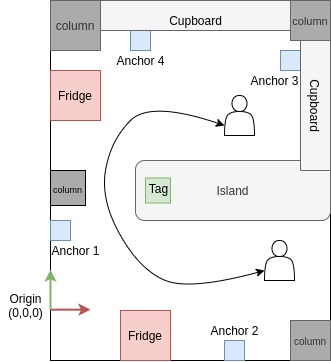
\includegraphics[scale=0.8]{Test_procedure}
    \caption{Path taken by person to randomly occlude anchors and tag.}
    \label{fig:occlude}
\end{figure}


\section{Stationary Tags}\label{sec:stationary-tags}
For the stationary tag tests, the tag was placed on a known point in the workspace and it was introduced to the basic limitations discussed in previous chapters.
The results for the loss of a single anchor was no different than the case recorded previously without the EKF.
However, Figure: ~\ref{fig:stat_anchors} shows the results obtained with the tags located at various positions whilst a person walks randomly in the environment.
In contrast to the previous section it can be seen the system with the current configuration and EKF is able to withstand NLOS between the anchors and the tag with minimal change in the perceived position.
However, it is evident that the system is now susceptible to a steady state error which is expected due to the Pozyx's integration with an IMU.
The tag's position will not change drastically and this error will be present as long as the tag is stationary.
The following sections will have the Pozyx time in motion so this error is expected to reduce.

\begin{figure}[h!]
    \centering
    \begin{subfigure}{0.49\textwidth}
            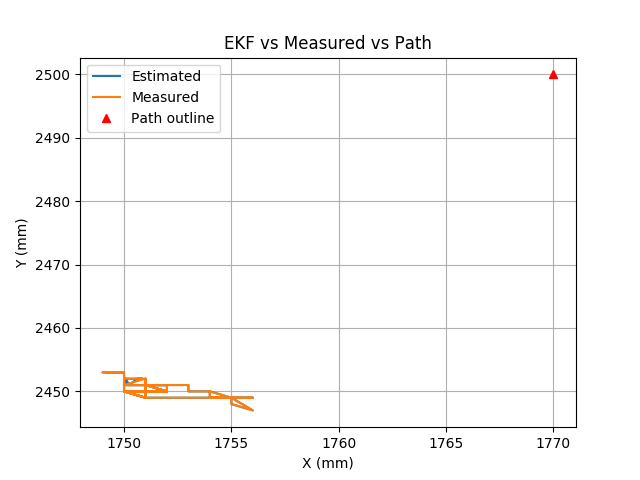
\includegraphics[width=\textwidth]{results/stationary_nlos_(1770,2500)}
            \caption{Result with tag at (1770,2500)}
    \end{subfigure}
    \begin{subfigure}{0.49\textwidth}
            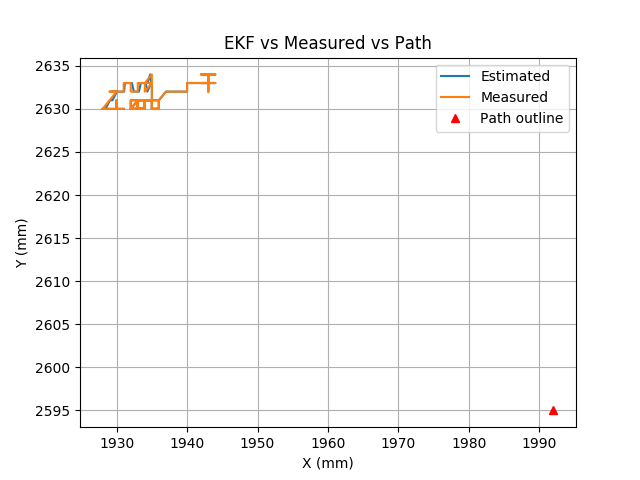
\includegraphics[width=\textwidth]{results/stationary_nlos_(1992,2595)}
            \caption{Result with tag at (1992,2595)}
    \end{subfigure}
    \begin{subfigure}{0.5\textwidth}
            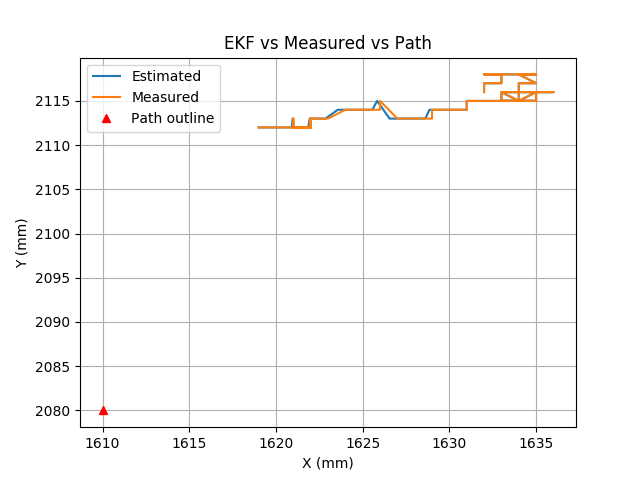
\includegraphics[width=\textwidth]{results/stationary_nlos_origin}
            \caption{Result with tag at (1610,2080)}
    \end{subfigure}
    \caption{Results obtained with NLOS and a single anchor.}
    \label{fig:stat_anchors}
\end{figure}
\newpage
\section{Person moving the tag}\label{sec:person-moving-the-tag}
Two trajectories were outlined for these subset of tests.
Table:~\ref{tb:trajs} shows the waypoints of each of the trajectories.
Trajectory one is a quadrilateral whilst trajectory two is a simply just a combination of straight line segments.
In these tests the tag was moved along the chosen trajectory whilst NLOS occurred randomly due to a person walking.
\begin{table}[ht!]
    \centering
    \begin{tabular}{|c|c|}
        \hline
        & Waypoints $(x,y)$(mm)\\
        \hline
        Trajectory 1 & $\begin{array}{c}
                            (1610, 2080)\\
                            (2111, 2080)\\
                            (1910, 2380)\\
                            (1610, 2580)\\
                            (1610, 2080)
        \end{array}$\\
        \hline
        Trajectory 2 & $\begin{array}{c}
                            (1610, 2080)\\
                            (1710, 2200)\\
                            (1760, 2300)\\
                            (1770, 2500)\\
                            (1840, 2580)\\
                            (1934, 2625)\\
                            (1992, 2595)
        \end{array}$\\
        \hline
    \end{tabular}
    \caption{Trajectories used in the tests for data collection.}
    \label{tb:trajs}
\end{table}
Figure:~\ref{fig:nlos_ppl} shows the paths recorded for each of these trajectories.
It can be seen that as expected the EKF smoothens the supposed trajectory providing a better estimate but it is unable to fully track the position of the tag in the environment.
\begin{figure}[h!]
    \centering
    \begin{subfigure}{0.7\textwidth}
            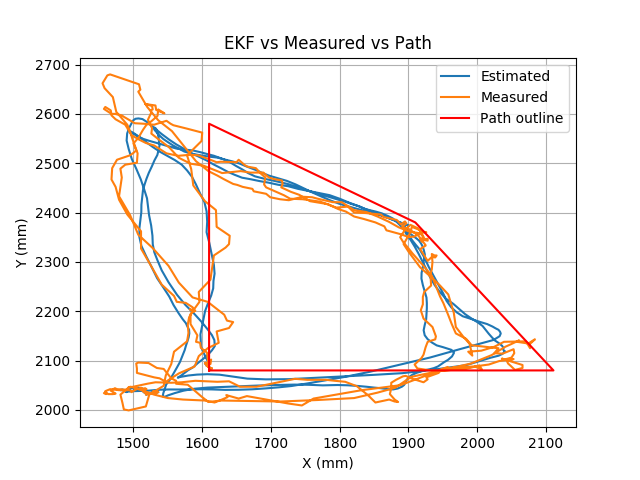
\includegraphics[width=\textwidth]{results/traingle_path_human(nlos)}
            \caption{Movement along Trajectory 1}
    \end{subfigure}
    \begin{subfigure}{0.7\textwidth}
            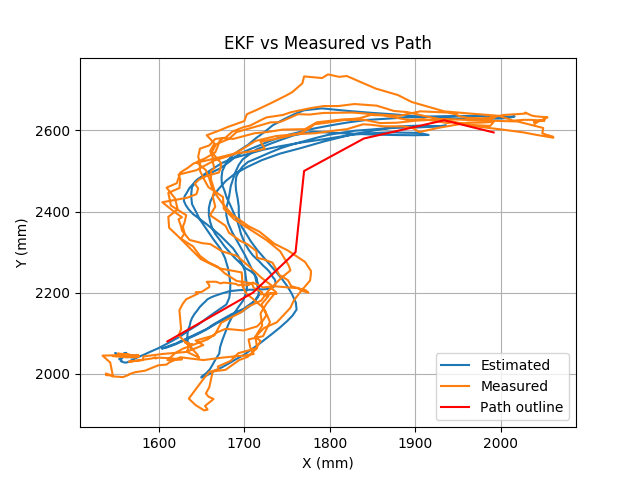
\includegraphics[width=\textwidth]{results/movement_along_c_path_human}
            \caption{Movement along Trajectory 2}
    \end{subfigure}
    \caption{Results obtained with NLOS and a single anchor.}
    \label{fig:nlos_ppl}
\end{figure}

%\lipsum[2-10]
